\chapter{Experiments}
\label{ch:intro}

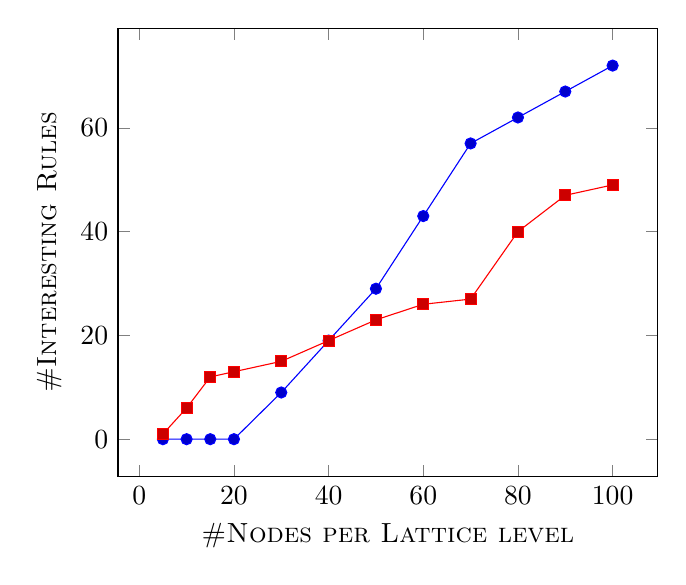
\begin{tikzpicture}[scale=1.0]
 \begin{axis}[
        xlabel=\textsc{\#Nodes per Lattice level},
        ylabel=\textsc{\#Interesting Rules}
    ]
\addplot coordinates {(5,0) (10,0) (15, 0) (20, 0) (30, 9) (40,19) (50,29) (60,43) (70,57) (80,62) (90,67) (100,72)};% (110,75) (120,79) (130,84) (140,88) (150,94) (200,122) (250,159) (300,178) (350,200) (400,214) (450,231) (500,242)};
\addplot coordinates {(5,1) (10,6) (15,12) (20,13) (30,15) (40,19) (50,23) (60,26) (70,27) (80,40) (90,47) (100,49)};% (110,) (120,) (130,) (140,) (150,) (200,) (250,) (300,) (350,) (400,) (450,) (500,)};

\end{axis}
\end{tikzpicture}


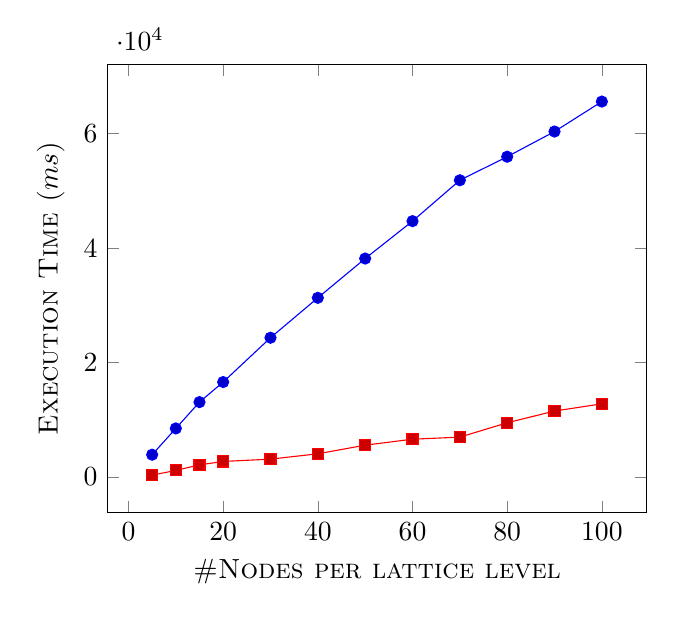
\begin{tikzpicture}[scale=1.0]
 \begin{axis}[
        xlabel=\textsc{\#Nodes per lattice level},
        ylabel=\textsc{Execution Time ($ms$)}
    ]
\addplot coordinates {(5,3905) (10,8496) (15,13097) (20,16601) (30,24348) (40,31322) (50,38189) (60,44724) (70,51869) (80,55981) (90,60382) (100,65622)};% (110,75) (120,79) (130,84) (140,88) (150,94) (200,122) (250,159) (300,178) (350,200) (400,214) (450,231) (500,242)};
\addplot coordinates {(5, 330) (10,1161) (15, 2128) (20, 2722) (30, 3130) (40, 4060) (50, 5571) (60, 6613) (70, 6976) (80, 9483) (90,11534) (100,12795)};% (110,) (120,) (130,) (140,) (150,) (200,) (250,) (300,) (350,) (400,) (450,) (500,)};

\end{axis}
\end{tikzpicture}

